\documentclass[journal,12pt,twocolumn]{article}
\usepackage[margin=0.5in]{geometry}
\usepackage[cmex10]{amsmath}
\usepackage{amsmath}
\usepackage{array}
\usepackage{booktabs}
% The preceding line is only needed to identify funding in the first footnote. If that is unneeded, please comment it out.
\usepackage{cite}
\usepackage{amsmath,amssymb,amsfonts}
\usepackage{graphicx}
\usepackage{textcomp}
\usepackage{xcolor}
\graphicspath{{./figs/}}{}
\usepackage{amsmath,amssymb,amsfonts,amsthm}
\usepackage{gensymb}
\newcommand{\myvec}[1]{\ensuremath{\begin{pmatrix}#1\end{pmatrix}}}

\let\vec\mathbf
\title{Matrix-Circle}
\author{SHREYASH CHANDRA PUTTA}
\begin{document}
\maketitle
\tableofcontents
\bigskip
\section{Problem Statement}
To find angle QPR of the triangle PQR which is inscribed in the circle $x^2 + y^2 = 25$. If Q and R  have  co-ordinates (3,4) and (-4,3) respectively .
\section{Construction}
 {\begin{table}[h]
    \centering
    \begin{tabular}{|c|c|c|}
       \hline
       \textbf{Symbol}&\textbf{Value}&\textbf{Description}  \\
       \hline
       $\vec{O}$ & $\myvec{
		    0\\
		    0}$
	    & Center point\\
        \hline
        $\vec{r}$ & 5
	    & Radius\\
        \hline
	    $\vec{Q}$ & $\myvec{
		    3\\
		    4}$
	    & given point\\
        \hline
	    $\vec{R}$ & $\myvec{-4\\3}$
 & given point\\
        \hline
	    $\vec{P}$ & $\myvec{rcos(\alpha)\\
  rsin(\alpha)}$
 & user defined point \\
       \hline
    \end{tabular}
    \caption{Parameters}
    \label{tab:my_label}
\end{table}}
 %%%%%%%%%%%
\begin{figure}[h]
    \centering
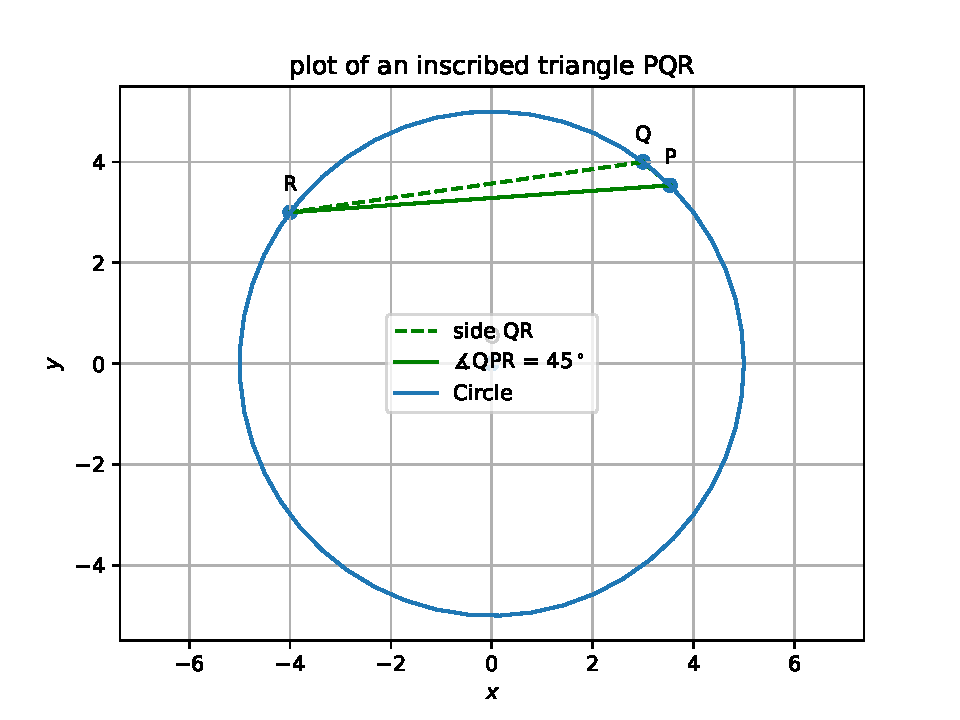
\includegraphics[width=\columnwidth]{fig/circlefig.pdf}
    \caption{triangle inscribed in Circle and its angle QPR }
    \label{fig:my_label}
\end{figure}
\vspace{0cm}
%%%%%%%%%%%%%%%%%%%%%%solution%%%%%%%%%%%%%%%%%%
\section{solution}
Given that Points given are on the circle forms an inscribed triangle the points $\vec{Q}$, $\vec{R}$ and any point$\vec{P}$ on the given circle   \\

The circle given,
 \begin{align}
    \label{eq:conic_quad_form}
    \vec{x}^{\top}\vec{x}=25
 \end{align}
From General Equation:
\begin{align}
    \label{eq:conic_quad_form}
    \vec{x}^{\top}\vec{x}+2\vec{u}^{\top}\vec{x}+f=0
    \end{align}
    
where
\begin{align}
	\label{eq:u_vector}
	\vec{u} &= -\myvec{0\\0},
	\\
	\label{eq:f_value}
	f &= -25	
\end{align}
%%%%%%%%%%%%%%%%%%%%%%%%%%%%%%%
Centre and Radius of given circle are :
\begin{align}
	\label{eq:V_matrix}
	\vec{O} = -\vec{u} = \myvec{0\\0}\\
	r = \sqrt{\vec{u}^{\top}\vec{u}-f} = 5
	 \label{eq-7} 
\end{align}
%%%%%%%%%%%%%%%%%%%%%%%%%%%%
\\
Point on the circle should satisfy the circle equation so, we take 
\begin{align}
\vec{P}=\myvec{rcos(\alpha)\\
  rsin(\alpha)}\\
 \vec{Q}=\myvec{3\\
  4}\\
   \vec{R}=\myvec{-4\\
  3}
\end{align}
\\
Considering $\vec{P}$,$\vec{Q}$and $\vec{R}$ as the Coordinates of the Inscribed Triangle
\\
\\
We know,
The direction vector of the line joining two points $\vec{A}$, $\vec{B}$ is given by
\begin{equation}
	\vec{m}=
     \vec{B}-  \vec{A}
  \label{eq-11}
\end{equation}
\\
we Know
The angle between two vectors is given by
\begin{equation}
\theta = {cos}^{-1}\frac{\vec{A^{\top}} \vec{B}}{\vec{\|A\| \|B\|}}
   \label{eq-12}
\end{equation}
\\
By the equations (\ref{eq-11}) and (\ref{eq-12}) for $\vec{\angle{QPR}}$ we consider,
\begin{equation}
	\vec{\measuredangle{QPR}} = {cos}^{-1}\frac{(\vec{P-Q})^{\top} (\vec{P-R})}{\vec{\|P-Q\| \|P-R\|}}
   \label{eq-14}
\end{equation}

\subsection{Case 1: Major Arc} If $\vec{P}$ lies on major Arc of the circle for given $\vec{Q}$ and $\vec{R}$ points
\begin{equation}
 \vec{\measuredangle{QPR}} = 45\degree
  \label{eq-14}
\end{equation}
\subsection{Case 2: Minor Arc}
If $\vec{P}$ lies on minor Arc of the circle for given $\vec{Q}$ and $\vec{R}$ points.
\begin{equation}
\vec{\measuredangle{QPR}} = 135\degree
\label{eq-15}
\end{equation}
where,$\vec{P}$ is a random point on the given circle for its $\boldsymbol{\alpha}$\\

\section{Software}

Download the following code using,\\
{\setlength\extrarowheight{2pt}
\begin{table}[h]
    \centering
    \begin{tabular}{|c|}
    \hline \\
         https://github.com/chanduputta/\\FWC-Module1Assignments/blob/\\main/circle/circle.py  \\ 
\hline
    \end{tabular}
\end{table}
}\\
and execute the code by using command\\
\centering
\textbf{cmd1}:Python3  circle.py\\
\textbf{cmd2}:Input your $\boldsymbol{\alpha}$ value (0 to 360\degree)
\section{Conclusion}

\begin{center}
We found the  $\vec{\measuredangle{QPR}} $ of the $\vec{\triangle{PQR}}$ which is inscribed in the circle $\vec{x^2 + y^2 = 25}$.
\\Where $\vec{P}$ is  point on the circle as 
\\i) $\textbf{45\degree}$, If $\vec{P}$ lies on Major Arc of Given Circle\\
ii) $\textbf{135\degree}$, If $\vec{P}$ lies on Minor Arc of Given Circle
\end{center}
\end{document}
